\subsection{Data}

\begin{figure}[h!]
\centering
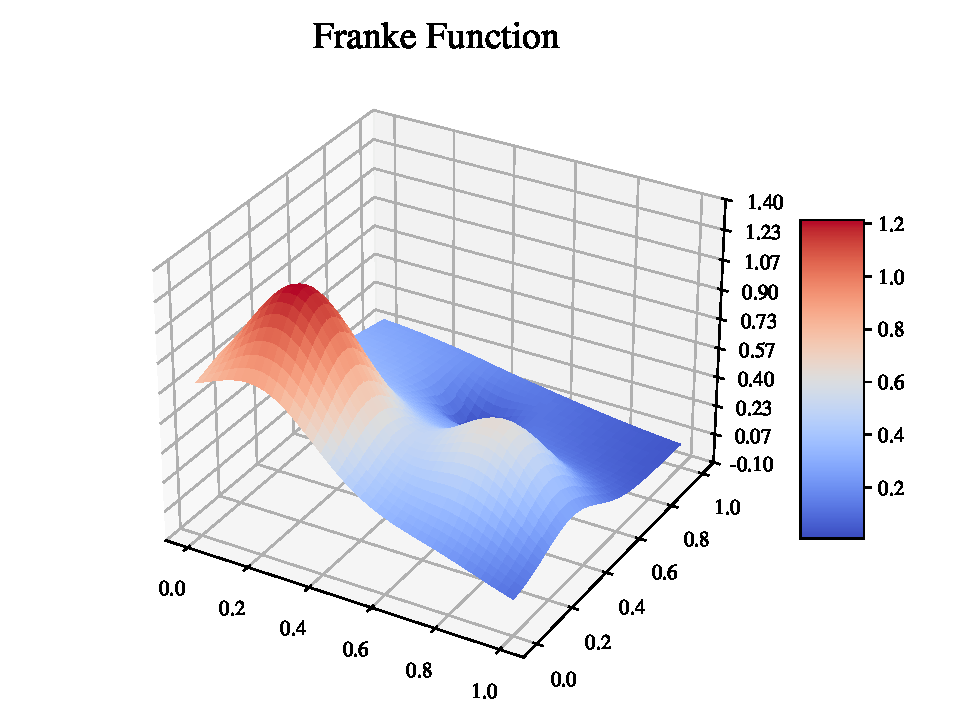
\includegraphics[width=1\linewidth]{project_1/figures/figures_in_report/franke_func.pdf}
\caption{Franke function for x,y $\in [0,1]$}
\label{franke}
\end{figure}

\subsubsection{Franke Function}
We first implement our methods on a synthetic data-set based on the Franke function \citep[p. 13]{frank}. Originally proposed by Richard Franke in 1979 is a much used function for testing linear regression and interpolation problems.
The Franke function is defined as:
\begin{align}\label{eq:franke}
    f(x, y) = &\frac{3}{4} \exp\left( -\frac{(9x - 2)^2}{4} - \frac{(9y - 2)^2}{4} \right) \nonumber \\
    + &\frac{3}{4} \exp\left( -\frac{(9x + 1)^2}{49} - \frac{(9y + 1)^2}{10} \right) \nonumber \\
    + &\frac{1}{2} \exp\left( -\frac{(9x - 7)^2}{4} - \frac{(9y - 3)^2}{4} \right) \nonumber \\
    - &\frac{1}{5} \exp\left( -(9x - 4)^2 - (9y - 7)^2 \right)
\end{align}
The Franke function is defined on $[0, 1]^2$, and produces a surface in the range $(0, 1.25)$ with two Gaussian peaks and a Gaussian dip, imposed on a surface sloping down towards $(x,y)=(1, 1)$ \citep[p. 13]{frank}.

\begin{figure}[h!]
\centering
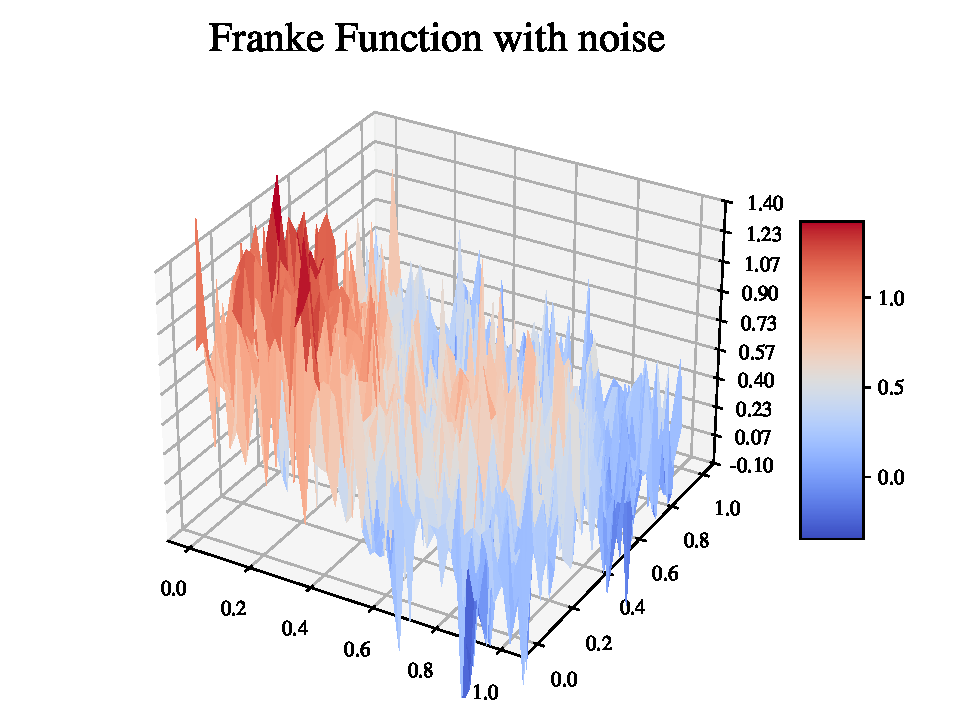
\includegraphics[width=1\linewidth]{project_1/figures/figures_in_report/franke_func_noise.pdf}
\caption{Franke function for x,y $\in [0,1]$ with added noise term: $(3/10) \mathcal{N}(0, 1)$.}
\label{fig:franke_noise}
\end{figure}

In order to enable potential overfitting in the models, we added a stochastic noise term to the Franke function. The noise term is generated using a normal distribution, and scaled by a factor of $0.3$. By choosing this noise term factor, we introduce sufficient amounts of noise to observe overfitting in some models, while maintaining the underlying structure to be recognized by the models (see Fig. \ref{fig:franke_noise}). Hence, we use the following function in our analysis:
\begin{align}\label{eq:franke_noise}
    f^*(x,y) = f(x, y) + \frac{3}{10} \mathcal{N}(0, 1),
\end{align}
where $f(x,y)$ is defined in Eq. \ref{eq:franke}. All subsequent references to the Franke function will mean the function defined in Eq. \ref{eq:franke_noise}.

For the Franke data, we use 41 data points along each axis, for a total of 1681 data point (i.e. $41^2$).

\subsubsection{Terrain data}

\begin{figure}
    \centering
    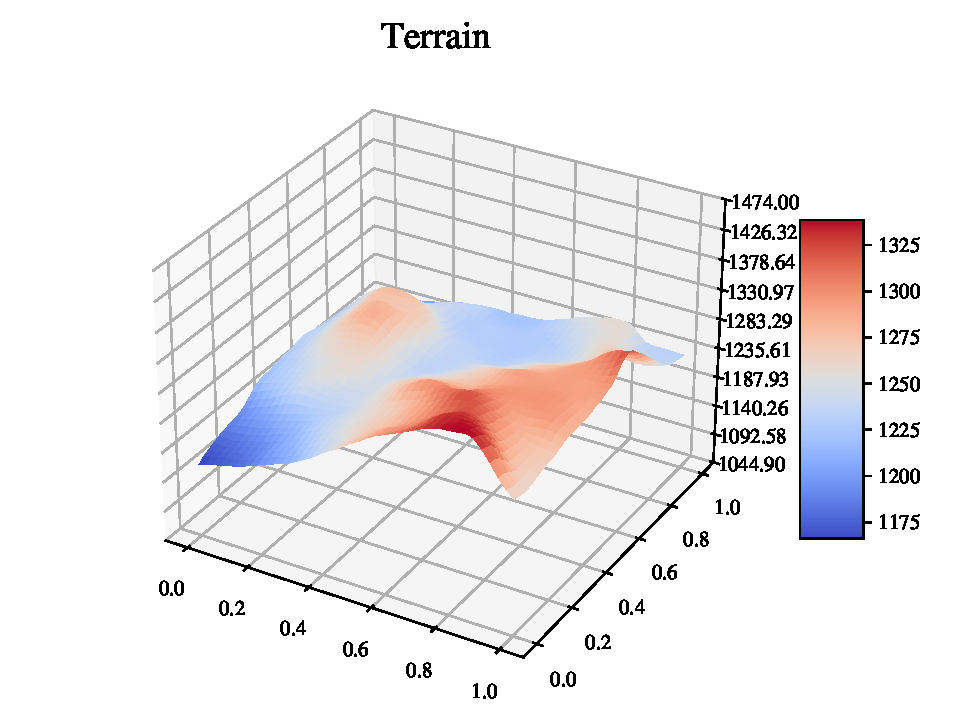
\includegraphics[width=1\linewidth]{project_1/figures/figures_in_report/terrain.pdf}
    \caption{Terrain data}
    \label{data:terrain}
\end{figure}

Secondly, we implement our methods on real terrain data \cite{mortengithub}. The data we use contain \mia{struggling to write when the data is just taken from GitHub, I know nothing about it...}

\mia{100 data points }

\subsubsection{Scaling and train/test-split}
To ensure our different models are trained and tested on the exact same data, making them comparable, we perform the train/test split of the data initially, in a separate data handling class.
After setting up our design matrix (\ref{design-matrix}), we scale it using the \texttt{StandardScaler} class from \textit{Scikit learn} \cite{sklearn}.
The data handling class also implements bootstrap sampling of the data, as well as splitting data in equally sized sets to use for cross validation.

\subsection{Implementation of models}
We implement a general \texttt{RegModel} class, with subclasses for each model type.
In these classes we implement functions for fitting the models on data (both simple data, and bootstrap and cross validation sets), performing predictions based on these fits, and calculating MSE and R\^2 for these models.

For both the Ordinary least squares and Ridge models we have implemented the fit and prediction function manually, through equations Eq. \ref{betaols} and Eq. \ref{pen} respectively.
As Lasso regression has no explicit formula to perform the fit, i.e. calculate the optimal coefficients, we utilize the \texttt{Lasso} class from \textit{Scikit learn} \cite{sklearn}.

\subsection{Hyperparameter selection}
All the linear model types in this project (OLS, Ridge and Lasso) have hyperparameters which results in different models. 
These hyperparameters are the model complexity (i.e. the maximum degree of $x$ and $y$ in the resulting expression) and the weight parameter for the regularization for Ridge and Lasso regression ($\lambda$). 
Optimizing the ordinary least squares model is simple, as we only need to test it on different model-complexity. 
We run a set of bootstrap samples for each degree complexity, and choose the model with the lowest MSE.

For Ridge and Lasso however, we require selecting two parameters simultaneously. As different model-complexities might obtain the best MSE at different values for $\lambda$, it does not suffice to lock one and test the other only for that value. 
We use grid search, a standard technique for tuning multiple hyper parameters \citep[p. 302]{grid_search}.
Grid search is an exhaustive search over a selection of values for each parameter. 
We perform two layers of grid search on each type of model and set of data. 
In the first layer we test model-complexities ranging from 1 to 11, and lambdas from $1*10^{-5}$ up to $9$ (with increasing step size according to order of magnitude). 
We use 200 bootstrap samples, and pick the values for complexity $d$ and $\lambda$ resulting in the lowest MSE. 
In the second layer, we use only the complexities $d-1,\ d,\ d+1$, and 40 different $\lambda$-values ranging from $(4/5)\lambda$ to $(6/5)\lambda$. 
We do this in order to fine tune our selections of hyper-parameters.
